
%% bare_jrnl.tex
%% V1.3
%% 2007/01/11
%% by Michael Shell
%% see http://www.michaelshell.org/
%% for current contact information.
%%
%% This is a skeleton file demonstrating the use of IEEEtran.cls
%% (requires IEEEtran.cls version 1.7 or later) with an IEEE journal paper.
%%
%% Support sites:
%% http://www.michaelshell.org/tex/ieeetran/
%% http://www.ctan.org/tex-archive/macros/latex/contrib/IEEEtran/
%% and
%% http://www.ieee.org/



% *** Authors should verify (and, if needed, correct) their LaTeX system  ***
% *** with the testflow diagnostic prior to trusting their LaTeX platform ***
% *** with production work. IEEE's font choices can trigger bugs that do  ***
% *** not appear when using other class files.                            ***
% The testflow support page is at:
% http://www.michaelshell.org/tex/testflow/


%%*************************************************************************
%% Legal Notice:
%% This code is offered as-is without any warranty either expressed or
%% implied; without even the implied warranty of MERCHANTABILITY or
%% FITNESS FOR A PARTICULAR PURPOSE! 
%% User assumes all risk.
%% In no event shall IEEE or any contributor to this code be liable for
%% any damages or losses, including, but not limited to, incidental,
%% consequential, or any other damages, resulting from the use or misuse
%% of any information contained here.
%%
%% All comments are the opinions of their respective authors and are not
%% necessarily endorsed by the IEEE.
%%
%% This work is distributed under the LaTeX Project Public License (LPPL)
%% ( http://www.latex-project.org/ ) version 1.3, and may be freely used,
%% distributed and modified. A copy of the LPPL, version 1.3, is included
%% in the base LaTeX documentation of all distributions of LaTeX released
%% 2003/12/01 or later.
%% Retain all contribution notices and credits.
%% ** Modified files should be clearly indicated as such, including  **
%% ** renaming them and changing author support contact information. **
%%
%% File list of work: IEEEtran.cls, IEEEtran_HOWTO.pdf, bare_adv.tex,
%%                    bare_conf.tex, bare_jrnl.tex, bare_jrnl_compsoc.tex
%%*************************************************************************

% Note that the a4paper option is mainly intended so that authors in
% countries using A4 can easily print to A4 and see how their papers will
% look in print - the typesetting of the document will not typically be
% affected with changes in paper size (but the bottom and side margins will).
% Use the testflow package mentioned above to verify correct handling of
% both paper sizes by the user's LaTeX system.
%
% Also note that the "draftcls" or "draftclsnofoot", not "draft", option
% should be used if it is desired that the figures are to be displayed in
% draft mode.
%
\documentclass[journal,twoside]{IEEEtran}
\usepackage{float}
\usepackage{graphicx}
\usepackage{caption}
\usepackage{subcaption}

\usepackage{array}

\usepackage{amsmath}
\usepackage{mathtools}
\DeclareMathOperator{\Hessian}{H}

% Some very useful LaTeX packages include:
% (uncomment the ones you want to load)


% *** MISC UTILITY PACKAGES ***
%
%\usepackage{ifpdf}
% Heiko Oberdiek's ifpdf.sty is very useful if you need conditional
% compilation based on whether the output is pdf or dvi.
% usage:
% \ifpdf
%   % pdf code
% \else
%   % dvi code
% \fi
% The latest version of ifpdf.sty can be obtained from:
% http://www.ctan.org/tex-archive/macros/latex/contrib/oberdiek/
% Also, note that IEEEtran.cls V1.7 and later provides a builtin
% \ifCLASSINFOpdf conditional that works the same way.
% When switching from latex to pdflatex and vice-versa, the compiler may
% have to be run twice to clear warning/error messages.






% *** CITATION PACKAGES ***
%
%\usepackage{cite}
% cite.sty was written by Donald Arseneau
% V1.6 and later of IEEEtran pre-defines the format of the cite.sty package
% \cite{} output to follow that of IEEE. Loading the cite package will
% result in citation numbers being automatically sorted and properly
% "compressed/ranged". e.g., [1], [9], [2], [7], [5], [6] without using
% cite.sty will become [1], [2], [5]--[7], [9] using cite.sty. cite.sty's
% \cite will automatically add leading space, if needed. Use cite.sty's
% noadjust option (cite.sty V3.8 and later) if you want to turn this off.
% cite.sty is already installed on most LaTeX systems. Be sure and use
% version 4.0 (2003-05-27) and later if using hyperref.sty. cite.sty does
% not currently provide for hyperlinked citations.
% The latest version can be obtained at:
% http://www.ctan.org/tex-archive/macros/latex/contrib/cite/
% The documentation is contained in the cite.sty file itself.






% *** GRAPHICS RELATED PACKAGES ***
%
\ifCLASSINFOpdf
  % \usepackage[pdftex]{graphicx}
  % declare the path(s) where your graphic files are
  % \graphicspath{{../pdf/}{../jpeg/}}
  % and their extensions so you won't have to specify these with
  % every instance of \includegraphics
  % \DeclareGraphicsExtensions{.pdf,.jpeg,.png}
\else
  % or other class option (dvipsone, dvipdf, if not using dvips). graphicx
  % will default to the driver specified in the system graphics.cfg if no
  % driver is specified.
  % \usepackage[dvips]{graphicx}
  % declare the path(s) where your graphic files are
  % \graphicspath{{../eps/}}
  % and their extensions so you won't have to specify these with
  % every instance of \includegraphics
  % \DeclareGraphicsExtensions{.eps}
\fi
% graphicx was written by David Carlisle and Sebastian Rahtz. It is
% required if you want graphics, photos, etc. graphicx.sty is already
% installed on most LaTeX systems. The latest version and documentation can
% be obtained at: 
% http://www.ctan.org/tex-archive/macros/latex/required/graphics/
% Another good source of documentation is "Using Imported Graphics in
% LaTeX2e" by Keith Reckdahl which can be found as epslatex.ps or
% epslatex.pdf at: http://www.ctan.org/tex-archive/info/
%
% latex, and pdflatex in dvi mode, support graphics in encapsulated
% postscript (.eps) format. pdflatex in pdf mode supports graphics
% in .pdf, .jpeg, .png and .mps (metapost) formats. Users should ensure
% that all non-photo figures use a vector format (.eps, .pdf, .mps) and
% not a bitmapped formats (.jpeg, .png). IEEE frowns on bitmapped formats
% which can result in "jaggedy"/blurry rendering of lines and letters as
% well as large increases in file sizes.
%
% You can find documentation about the pdfTeX application at:
% http://www.tug.org/applications/pdftex





% *** MATH PACKAGES ***
%
%\usepackage[cmex10]{amsmath}
% A popular package from the American Mathematical Society that provides
% many useful and powerful commands for dealing with mathematics. If using
% it, be sure to load this package with the cmex10 option to ensure that
% only type 1 fonts will utilized at all point sizes. Without this option,
% it is possible that some math symbols, particularly those within
% footnotes, will be rendered in bitmap form which will result in a
% document that can not be IEEE Xplore compliant!
%
% Also, note that the amsmath package sets \interdisplaylinepenalty to 10000
% thus preventing page breaks from occurring within multiline equations. Use:
%\interdisplaylinepenalty=2500
% after loading amsmath to restore such page breaks as IEEEtran.cls normally
% does. amsmath.sty is already installed on most LaTeX systems. The latest
% version and documentation can be obtained at:
% http://www.ctan.org/tex-archive/macros/latex/required/amslatex/math/





% *** SPECIALIZED LIST PACKAGES ***
%
%\usepackage{algorithmic}
% algorithmic.sty was written by Peter Williams and Rogerio Brito.
% This package provides an algorithmic environment fo describing algorithms.
% You can use the algorithmic environment in-text or within a figure
% environment to provide for a floating algorithm. Do NOT use the algorithm
% floating environment provided by algorithm.sty (by the same authors) or
% algorithm2e.sty (by Christophe Fiorio) as IEEE does not use dedicated
% algorithm float types and packages that provide these will not provide
% correct IEEE style captions. The latest version and documentation of
% algorithmic.sty can be obtained at:
% http://www.ctan.org/tex-archive/macros/latex/contrib/algorithms/
% There is also a support site at:
% http://algorithms.berlios.de/index.html
% Also of interest may be the (relatively newer and more customizable)
% algorithmicx.sty package by Szasz Janos:
% http://www.ctan.org/tex-archive/macros/latex/contrib/algorithmicx/




% *** ALIGNMENT PACKAGES ***
%
%\usepackage{array}
% Frank Mittelbach's and David Carlisle's array.sty patches and improves
% the standard LaTeX2e array and tabular environments to provide better
% appearance and additional user controls. As the default LaTeX2e table
% generation code is lacking to the point of almost being broken with
% respect to the quality of the end results, all users are strongly
% advised to use an enhanced (at the very least that provided by array.sty)
% set of table tools. array.sty is already installed on most systems. The
% latest version and documentation can be obtained at:
% http://www.ctan.org/tex-archive/macros/latex/required/tools/


%\usepackage{mdwmath}
%\usepackage{mdwtab}
% Also highly recommended is Mark Wooding's extremely powerful MDW tools,
% especially mdwmath.sty and mdwtab.sty which are used to format equations
% and tables, respectively. The MDWtools set is already installed on most
% LaTeX systems. The lastest version and documentation is available at:
% http://www.ctan.org/tex-archive/macros/latex/contrib/mdwtools/


% IEEEtran contains the IEEEeqnarray family of commands that can be used to
% generate multiline equations as well as matrices, tables, etc., of high
% quality.


%\usepackage{eqparbox}
% Also of notable interest is Scott Pakin's eqparbox package for creating
% (automatically sized) equal width boxes - aka "natural width parboxes".
% Available at:
% http://www.ctan.org/tex-archive/macros/latex/contrib/eqparbox/





% *** SUBFIGURE PACKAGES ***
%\usepackage[tight,footnotesize]{subfigure}
% subfigure.sty was written by Steven Douglas Cochran. This package makes it
% easy to put subfigures in your figures. e.g., "Figure 1a and 1b". For IEEE
% work, it is a good idea to load it with the tight package option to reduce
% the amount of white space around the subfigures. subfigure.sty is already
% installed on most LaTeX systems. The latest version and documentation can
% be obtained at:
% http://www.ctan.org/tex-archive/obsolete/macros/latex/contrib/subfigure/
% subfigure.sty has been superceeded by subfig.sty.



%\usepackage[caption=false]{caption}
%\usepackage[font=footnotesize]{subfig}
% subfig.sty, also written by Steven Douglas Cochran, is the modern
% replacement for subfigure.sty. However, subfig.sty requires and
% automatically loads Axel Sommerfeldt's caption.sty which will override
% IEEEtran.cls handling of captions and this will result in nonIEEE style
% figure/table captions. To prevent this problem, be sure and preload
% caption.sty with its "caption=false" package option. This is will preserve
% IEEEtran.cls handing of captions. Version 1.3 (2005/06/28) and later 
% (recommended due to many improvements over 1.2) of subfig.sty supports
% the caption=false option directly:
%\usepackage[caption=false,font=footnotesize]{subfig}
%
% The latest version and documentation can be obtained at:
% http://www.ctan.org/tex-archive/macros/latex/contrib/subfig/
% The latest version and documentation of caption.sty can be obtained at:
% http://www.ctan.org/tex-archive/macros/latex/contrib/caption/




% *** FLOAT PACKAGES ***
%
%\usepackage{fixltx2e}
% fixltx2e, the successor to the earlier fix2col.sty, was written by
% Frank Mittelbach and David Carlisle. This package corrects a few problems
% in the LaTeX2e kernel, the most notable of which is that in current
% LaTeX2e releases, the ordering of single and double column floats is not
% guaranteed to be preserved. Thus, an unpatched LaTeX2e can allow a
% single column figure to be placed prior to an earlier double column
% figure. The latest version and documentation can be found at:
% http://www.ctan.org/tex-archive/macros/latex/base/



%\usepackage{stfloats}
% stfloats.sty was written by Sigitas Tolusis. This package gives LaTeX2e
% the ability to do double column floats at the bottom of the page as well
% as the top. (e.g., "\begin{figure*}[!b]" is not normally possible in
% LaTeX2e). It also provides a command:
%\fnbelowfloat
% to enable the placement of footnotes below bottom floats (the standard
% LaTeX2e kernel puts them above bottom floats). This is an invasive package
% which rewrites many portions of the LaTeX2e float routines. It may not work
% with other packages that modify the LaTeX2e float routines. The latest
% version and documentation can be obtained at:
% http://www.ctan.org/tex-archive/macros/latex/contrib/sttools/
% Documentation is contained in the stfloats.sty comments as well as in the
% presfull.pdf file. Do not use the stfloats baselinefloat ability as IEEE
% does not allow \baselineskip to stretch. Authors submitting work to the
% IEEE should note that IEEE rarely uses double column equations and
% that authors should try to avoid such use. Do not be tempted to use the
% cuted.sty or midfloat.sty packages (also by Sigitas Tolusis) as IEEE does
% not format its papers in such ways.


%\ifCLASSOPTIONcaptionsoff
%  \usepackage[nomarkers]{endfloat}
% \let\MYoriglatexcaption\caption
% \renewcommand{\caption}[2][\relax]{\MYoriglatexcaption[#2]{#2}}
%\fi
% endfloat.sty was written by James Darrell McCauley and Jeff Goldberg.
% This package may be useful when used in conjunction with IEEEtran.cls'
% captionsoff option. Some IEEE journals/societies require that submissions
% have lists of figures/tables at the end of the paper and that
% figures/tables without any captions are placed on a page by themselves at
% the end of the document. If needed, the draftcls IEEEtran class option or
% \CLASSINPUTbaselinestretch interface can be used to increase the line
% spacing as well. Be sure and use the nomarkers option of endfloat to
% prevent endfloat from "marking" where the figures would have been placed
% in the text. The two hack lines of code above are a slight modification of
% that suggested by in the endfloat docs (section 8.3.1) to ensure that
% the full captions always appear in the list of figures/tables - even if
% the user used the short optional argument of \caption[]{}.
% IEEE papers do not typically make use of \caption[]'s optional argument,
% so this should not be an issue. A similar trick can be used to disable
% captions of packages such as subfig.sty that lack options to turn off
% the subcaptions:
% For subfig.sty:
% \let\MYorigsubfloat\subfloat
% \renewcommand{\subfloat}[2][\relax]{\MYorigsubfloat[]{#2}}
% For subfigure.sty:
% \let\MYorigsubfigure\subfigure
% \renewcommand{\subfigure}[2][\relax]{\MYorigsubfigure[]{#2}}
% However, the above trick will not work if both optional arguments of
% the \subfloat/subfig command are used. Furthermore, there needs to be a
% description of each subfigure *somewhere* and endfloat does not add
% subfigure captions to its list of figures. Thus, the best approach is to
% avoid the use of subfigure captions (many IEEE journals avoid them anyway)
% and instead reference/explain all the subfigures within the main caption.
% The latest version of endfloat.sty and its documentation can obtained at:
% http://www.ctan.org/tex-archive/macros/latex/contrib/endfloat/
%
% The IEEEtran \ifCLASSOPTIONcaptionsoff conditional can also be used
% later in the document, say, to conditionally put the References on a 
% page by themselves.





% *** PDF, URL AND HYPERLINK PACKAGES ***
%
%\usepackage{url}
% url.sty was written by Donald Arseneau. It provides better support for
% handling and breaking URLs. url.sty is already installed on most LaTeX
% systems. The latest version can be obtained at:
% http://www.ctan.org/tex-archive/macros/latex/contrib/misc/
% Read the url.sty source comments for usage information. Basically,
% \url{my_url_here}.





% *** Do not adjust lengths that control margins, column widths, etc. ***
% *** Do not use packages that alter fonts (such as pslatex).         ***
% There should be no need to do such things with IEEEtran.cls V1.6 and later.
% (Unless specifically asked to do so by the journal or conference you plan
% to submit to, of course. )


% correct bad hyphenation here
\hyphenation{op-tical net-works semi-conduc-tor}


\begin{document}
\setcounter{page}{31}
%
% paper title
% can use linebreaks \\ within to get better formatting as desired
\title{Prototyping of a Voice Command Based Object Recognizing Robot Using Speech and Image Feature Extraction}
%
%
% author names and IEEE memberships
% note positions of commas and nonbreaking spaces ( ~ ) LaTeX will not break
% a structure at a ~ so this keeps an author's name from being broken across
% two lines.
% use \thanks{} to gain access to the first footnote area
% a separate \thanks must be used for each paragraph as LaTeX2e's \thanks
% was not built to handle multiple paragraphs
%

\author{
    Bishal~Heuju\IEEEauthorrefmark{1},
   Bishal~Lakha, 
   Dipkamal~Bhusal, 
   Kanhaiya~Lal~Shrestha 
   and Nanda Bikram Adhikari\\
  Department of Electronics and Computer Engineering\\
  \textit{Institute of Engineering, Pulchowk, Lalitpur}\\
  b.heuju@gmail.com\IEEEauthorrefmark{1}
}

% note the % following the last \IEEEmembership and also \thanks - 
% these prevent an unwanted space from occurring between the last author name
% and the end of the author line. i.e., if you had this:
% 
% \author{....lastname \thanks{...} \thanks{...} }
%                     ^------------^------------^----Do not want these spaces!
%
% a space would be appended to the last name and could cause every name on that
% line to be shifted left slightly. This is one of those "LaTeX things". For
% instance, "\textbf{A} \textbf{B}" will typeset as "A B" not "AB". To get
% "AB" then you have to do: "\textbf{A}\textbf{B}"
% \thanks is no different in this regard, so shield the last } of each \thanks
% that ends a line with a % and do not let a space in before the next \thanks.
% Spaces after \IEEEmembership other than the last one are OK (and needed) as
% you are supposed to have spaces between the names. For what it is worth,
% this is a minor point as most people would not even notice if the said evil
% space somehow managed to creep in.



% The paper headers
\markboth{Zerone Scholar,~Vol.~1, No.~1, November~2016}%
{Heuju \MakeLowercase{\textit{et al.}}: Prototyping of a Voice Command Based Object Recognizing Robot}
% The only time the second header will appear is for the odd numbered pages
% after the title page when using the twoside option.
% 
% *** Note that you probably will NOT want to include the author's ***
% *** name in the headers of peer review papers.                   ***
% You can use \ifCLASSOPTIONpeerreview for conditional compilation here if
% you desire.




% If you want to put a publisher's ID mark on the page you can do it like
% this:
%\IEEEpubid{0000--0000/00\$00.00~\copyright~2007 IEEE}
% Remember, if you use this you must call \IEEEpubidadjcol in the second
% column for its text to clear the IEEEpubid mark.



% use for special paper notices
%\IEEEspecialpapernotice{(Invited Paper)}




% make the title area
\maketitle


\begin{abstract}
%\boldmath
    This paper describes the interfacing of two
    important human sensing features – hearing and vision, to a
    robot. The robot’s task is defined to recognize the voice
    command from the human and recognize the object that the
    robot has been commanded to recognize. The robot makes use of
    feature extraction from speech signals and images to recognize
    the given signal. The features from speech signals are extracted
    as Mel Frequency Cepstral Coefficients (MFCC); and the
    features from the image are extracted as Speeded Up Robust
    Features (SURF).
\end{abstract}
% IEEEtran.cls defaults to using nonbold math in the Abstract.
% This preserves the distinction between vectors and scalars. However,
% if the journal you are submitting to favors bold math in the abstract,
% then you can use LaTeX's standard command \boldmath at the very start
% of the abstract to achieve this. Many IEEE journals frown on math
% in the abstract anyway.

% Note that keywords are not normally used for peerreview papers.
\begin{IEEEkeywords}
    Embedded system, Object recognition, Robot vision system, Service robots, Speech recognition
\end{IEEEkeywords}






% For peer review papers, you can put extra information on the cover
% page as needed:
% \ifCLASSOPTIONpeerreview
% \begin{center} \bfseries EDICS Category: 3-BBND \end{center}
% \fi
%
% For peerreview papers, this IEEEtran command inserts a page break and
% creates the second title. It will be ignored for other modes.
\IEEEpeerreviewmaketitle



\section{Introduction}

The term robot generally connotes some anthropomorphic
appearance that has human-like perception. Among the
five classical human senses, hearing and vision are indeed the
two most useful senses. Here, we target to interface these two
senses into robots.

Technologists have confidently predicted the imminent
revolution in domestic and service robotics. We are told robots
will lift the burden of work from our homes and offices.
Robots will recognize their owners by appearance and voice.
We will give simple commands such as “Bring the coffee”,
and our robots will have the necessary sensing and intelligence
to fulfill the request. Eventually, robots will roam freely
around our homes and offices to help in whatever way they
see fit.

While the above scenario is still somewhat fantasy, the
steady development in the field of robotics and artificial
intelligence has made the possibilities of such robots seem
even closer and more compelling.

This project’s key concept lies in implementing the
fundamental idea of such robots - to recognize a voice
command and recognize objects and then execute the
commands. Through speech processing and image processing
algorithms, the robot can act like an intelligent assistant.

\section{Object Recognition}

Object recognition is a process for identifying a specific
object in a digital image or video. Object recognition
algorithms rely on matching, learning, or pattern recognition
algorithms using appearance-based or feature-based
techniques. Object recognition can be done using variety of
models, including:

\begin{itemize}
    \item Template matching \cite{Ahuja2013}
    \item Image segmentation and blob analysis \cite{Jia2008}
    \item Bag-of-words models with features such as SURF \cite{Schmitt2011}
    \item Gradient-based and derivative-based matching approaches \cite{Lecun1999}
\end{itemize}

Here we use the ‘Bag-of-words models with SURF’. This
model matches the features of the test image with the
database. It does not require all the features to match, and
hence the approach is more robust to occlusion and cluttered
background than other approaches.

\subsection{Object detection versus object recognition}

Frequently the terms “object detection” and “object
recognition” are used interchangeably and often mistaken to
be the same thing. There is a distinct difference between the two.

Object detection refers to detecting the presence of a
particular object in a given scene. We do not know what the
object might be.

Object recognition identifies an object in the given image.
For instance, object recognition system can tell if the given
image contains a cup or a pen, while the object detection
system can only tell if there is an object in the image but not a
pen.

\subsection{Bag-of-words}

In Bag of Words model, each image is represented as a
histogram of visual words. In this model, an image is
considered to be a document and patches of it are considered
words. The Bag of Words technique involves feature
detection, feature description and codebook generation. \cite{Grauman2011}

We applied SURF algorithm for feature detection and
description. In SURF, images are analyzed at different scales
in order to guarantee invariance in change of scale. Then the 2
detected interest points are provided with rotation and scale
invariant descriptor. SURF combines Hessian-Laplace 
region detector with its own gradient orientation-based feature
descriptor. \cite{Bay2006}

The Hessian matrix, H(x, \(\sigma\)), used to find interest points is
given in (1). It comprises second order partial derivatives. The
determinant of Hessian matrix, \(Det(H_{approx}\) ), (2) expresses
the extent of the response and is an expression of the local
change around the area. The hessian matrix is given as:

    \begin{align}
        \Hessian\left( x,\sigma \right) &= 
        \begin{bmatrix}
            L_{xx}\left( x,\sigma \right) & L_{xy}\left( x,\sigma\right) \\
            L_{xy}\left( x,\sigma\right) & L_{yy}\left( x,\sigma\right)
        \end{bmatrix}
    \end{align}

    where \(L_{xx}\left(x, \sigma\right)\), \(L_{xy}\left(x, \sigma\right)\), \(L_{yy}\left(x, \sigma\right)\) 
    are the convolution of the Gaussian second derivative \(\frac{\delta^2}{\delta x^2}g\left(\sigma\right)\) with the image I in point x. 
    The Gaussian kernels used for the hessian matrix
    must be discretized and cropped before we can apply them.
    The SURF algorithm approximates these kernels with
    rectangular boxes, box filters which makes it possible to
    calculate the approximated convolution effectively for
    arbitrarily sized kernel utilizing the integral image.

    \begin{equation}
        Det(H_{approx})=D_{xx}D_{yy} - (wD_{xy})^2
    \end{equation}

    The approximated and discrete kernels are referred to as
    \(D_{yy}\) for \(L_{yy}(x, \sigma)\) and \(D_{xy}\) for \(L_{xy} (x, \sigma)\). \cite{Bay2006}

    Thus obtained interest points are then used to find
    descriptors. The descriptor used in SURF describes the
    intensity content within the interest point neighborhood based
    on first order Haar wavelet \cite{Grauman2011} response in x and y direction.
    Interest point description begins with fixing a reproducible
    orientation based on information from a circular region and
    the interest point. Then a square region aligned to the selected
    orientation is constructed and then SURF descriptor is
    extracted.

\begin{figure}[!b]
    \begin{minipage}[t]{.45\linewidth}
        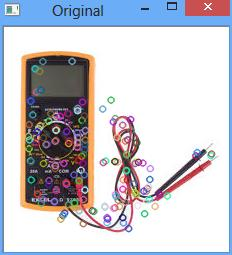
\includegraphics[width=\linewidth]{figure1a}
    \end{minipage}%
        \hfill%
    \begin{minipage}[t]{.45\linewidth}
        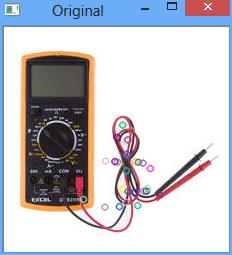
\includegraphics[width=\linewidth]{figure1b}
    \end{minipage}%
    \caption{SURF keypoints detection for different Hessian thresholds, 1000 (left) and 8000 (right)}
    \label{fig:figure1}
\end{figure}


    We then used the descriptors for codebook generation.
    Codebook is a collection of code words. Code words can be
    considered as representative of several similar patches. \cite{Minichino2015} We
    obtained the code words by performing k-means clustering
    over all feature vectors.

    \textit{K -means} is a very simple clustering algorithm that tries to
    partition the input data in k clusters. K -means works by
    iteratively refining an initial estimate of class centroids as
    follows:
    \begin{itemize}
        \item Initialize centroids \(\mu_i\) , \textit{i = 1 . . . k} , randomly or with some guess.
        \item Assign each data point to the class \(c_i\) of its nearest centroid.
    \item Update the centroids as the average of all data points assigned to that class.
    \item Repeat 2 and 3 until convergence.
\end{itemize}
K -means tries to minimize the total \textit{within-class} variance, \textit{V}

\begin{equation}
    V = \displaystyle\sum_{i=1}^{k}\sum_{x_j \in c_i}(x_j - u_i)^2
\end{equation}

where \(x_j\) are the data vectors. The algorithm above is a
heuristic refinement algorithm that works fine for most cases
but does not guarantee that the best solution is found. To avoid
the effects of choosing a bad centroid initialization, the
algorithm is often run several times with different
initialization centroids. Then the solution with lowest variance
\textit{V} is selected. The main drawback of this algorithm is that the
number of clusters needs to be decided beforehand and an
inappropriate choice will give poor clustering results. The
benefits are that it is simple to implement, it is parallelizable
and works well for a large range of problems without any need
for tuning. \cite{Alpaydin2010}

\begin{figure}[htb]
\centering
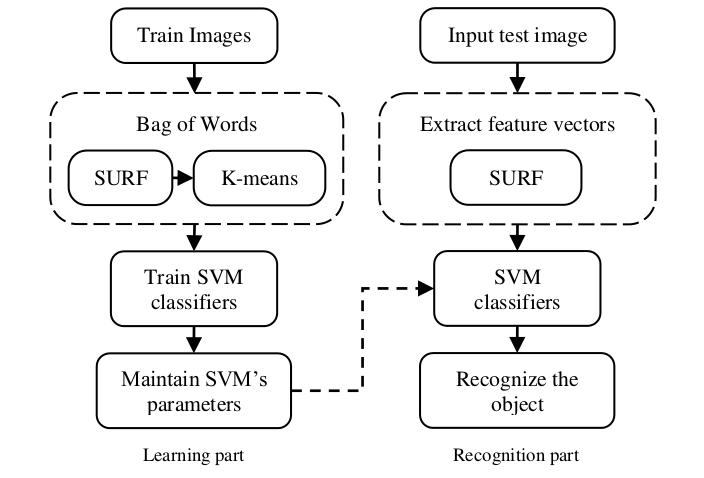
\includegraphics[width=3.0in]{figure2}
\caption{Block Diagram of Object Recognition}
\label{fig:figure2}
\end{figure}

\subsection{SVM Classifier}

A Support Vector Machine (SVM) is a discriminative
classifier formally defined by a separating hyperplane. The
operation of the SVM algorithm is based on finding the
hyperplane that gives the largest minimum distance to the
training examples. Twice, this distance receives the important
name of margin within SVM's theory. Therefore, the optimal
separating hyperplane maximizes the margin of the training
data. \cite{OpenCV2016}

\begin{figure}[htb]
\centering
\includegraphics[width=2.0in]{figure3}
\caption{Multimeter recognized by SVM Classifier}
\label{fig:figure3}
\end{figure}

There might exist multiple hyperplanes that offers a
solution to the problem. The SVM algorithm finds the optimal
hyperplane for the problem as in Fig 4.

\begin{figure}[H]
\centering
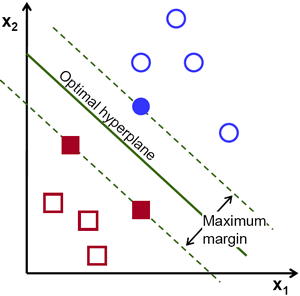
\includegraphics[width=2.0in]{figure4}
\caption{Optimal hyperplane separating two sets of data}
\label{fig:figure4}
\end{figure}

\section{Speech Recognition}

Speech recognition is one where the word (isolated or
continuous) is recognized by the system. This can be
performed by extracting the feature of the voice and
comparing with the known voice print (model of the system),
the acoustic signal of the human speech thus has to be
converted into electrical signal and then transformed into
coding patterns. Among various methods of the recognition
system, template matching has been extensively used. all
speaker recognition systems contain two main modules feature
extraction (model generation) and feature matching (template
matching). Feature extraction is the process that extracts a
small amount of data from the voice signal that can later be
used to represent each word. The average of the feature vector
is considered as the isolated-word-model. Feature matching
involves the actual procedure to identify the unknown speech
by comparing extracted features from his/her voice input with
the ones from a set of known words. \cite{Holmes2001} The overall process
of implementation of Speech recognition is as in Fig 5.

\begin{figure}[H]
\centering
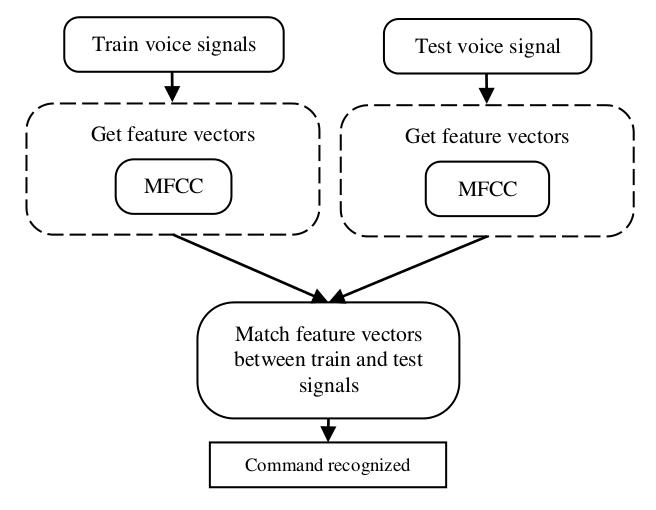
\includegraphics[width=3.0in]{figure5}
\caption{Block Diagram of Speech Recognition}
\label{fig:figure5}
\end{figure}

MFCC is based on human hearing perceptions which cannot
perceive frequencies over 1Khz. In other words, in MFCC is
based on known variation of the human ear’s critical
bandwidth with frequency. MFCC has two types of filter
which are spaced linearly at low frequency below 1000 Hz
and logarithmic spacing above 1000Hz. A subjective pitch is
present on Mel Frequency Scale to capture important
characteristic of phonetic in speech. \cite{Gopi2014}

\begin{figure}[H]
\centering
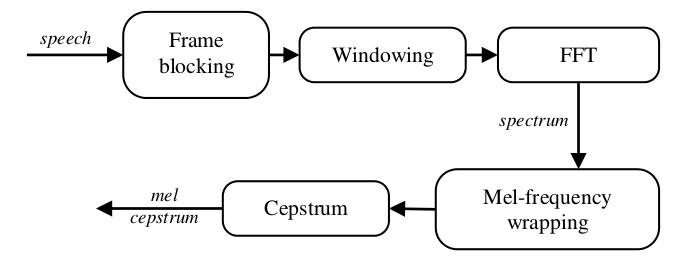
\includegraphics[width=3.5in]{figure6}
\caption{Block Diagram of MFCC}
\label{fig:figure6}
\end{figure}

\section{Voice Command Based Object Recognition}

In this section, we interface the speech recognition and
object recognition algorithms and their implementation in
Raspberry Pi.

\subsection{Raspberry Pi}
Raspberry Pi is a series of mini single board computers
developed by Raspberry Pi Foundation with the intent to
promote teaching of basic computer science in schools and
developing countries. In our context, the Raspberry Pi bears
the potential for image processing and speech processing. The
use of Raspberry Pi over an actual desktop or laptop PC is
chosen so as to make the robot an embedded system.
Raspberry Pi 2 has a quad-core 900MHz ARM Cortex-A7
chip with 1GB RAM. Python and OpenCV image processing
library are used for fulfilling our task. \cite{Raspberry2016}

\subsection{Camera Interface}
The Raspberry Pi also includes an on-board Camera Serial
Interface (CSI) port for connecting a 5MP, HD Raspberry Pi
Camera, which provides a viable option for using the camera
for image processing. The CSI bus is capable of extremely
high data rates, and it exclusively carries pixel data to the
processor. \cite{Camera2016}

\subsection{Speech and Object Recognition Interface}

Both the speech and object recognition algorithms are
implemented in the Raspberry Pi. The Raspberry Pi provides
enough horsepower to perform the recognition within it. The
speech processing and image processing tasks may run
simultaneously or in succession. Simple voice commands such
as ‘front’, ‘back’ will cause only the speech processing to take
action and send resulting control signals to the robot control
system. Other voice commands such as ‘recognize’, ‘follow’
will first cause speech recognition to take place to determine
the need of image processing. Then immediately after the
command is recognized, image processing comes into action.
The processed image signals generate required control signals
for the robot control system if necessary.

\begin{figure}[H]
\centering
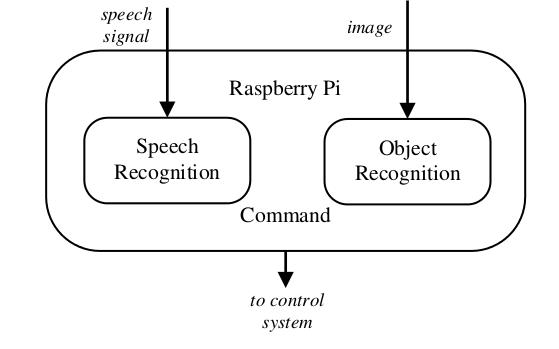
\includegraphics[width=3.2in]{figure7}
\caption{Interfacing of speech recognition and object recognition}
\label{fig:figure7}
\end{figure}

\section{Hardware Implementation}
The physical movement of the robot is controlled by a
separate microcontroller. The microcontroller used is
Atmega32. The microcontroller receives the control signals
through its serial port from the Raspberry Pi, and acts
accordingly as instructed by the Raspberry Pi to the
microcontroller.

\begin{figure}[htbp]
\centering
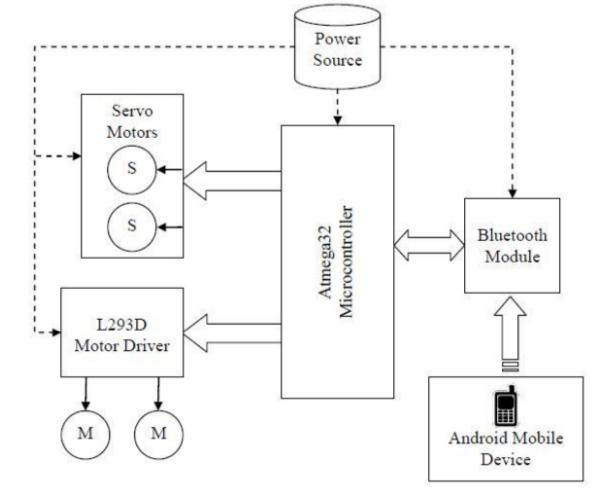
\includegraphics[width=3.2in]{figure8}
\caption{Robot control system block diagram}
\label{fig:figure8}
\end{figure}

Fig 8 represents the control system of the robot. It includes
two servo motors, denoted by ‘S’, which provides the pan and
tilt motion to the head of the robot that mounts the camera.
The two motors, denoted by ‘M’, provides the actual
movement of the robot body in the environment. The
simulation circuit of the system is shown in Fig 9.

The signals from the Raspberry Pi are generated based on
the speech and image processing. Based on the speech signals
and image signals, necessary commands are generated and
sent as control signals to the control system.

As an example: To track an object, the speech signal
‘follow’ is fed into the Raspberry Pi. This signal is processed
and recognized, and the robot captures the image of the object
in front of it in order to get prepared for tracking it. The robot
then starts to track the object and sends its position as control
signal to the control system. Based on the control signals, the
robot will move its head of whole body depending upon the
necessity.

\begin{figure}[htbp]
\centering
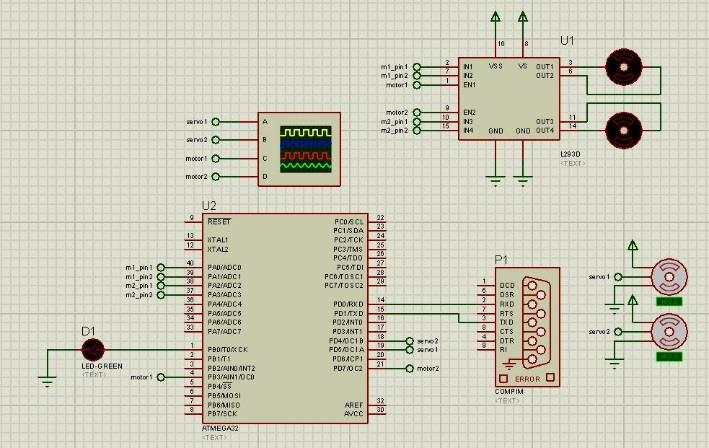
\includegraphics[width=3.2in]{figure9}
\caption{Simulation of the robot control system in Proteus}
\label{fig:figure9}
\end{figure}

\section{Experiment}
Here we mention the experiments that were conducted with
our developed system and discuss the results obtained from
them.

\subsection{Data Collection}
For training the object recognizer we collected a set of 50
images for each of the five different objects (calculator, key,
multimeter, watch, bottle). The training image-set in total
consists 250 images for training the classifier.

\subsection{Result}

\subsubsection{ Results of Object Recognition}
The trained classifier was used recognize different objects
present in an image. Different images containing one of the
trained objects was used to test the classifier. The recognition
efficiency of the classifier was obtained as in Table 1.

\begin{center}
    \begin{tabular}{| c | c |}
        \hline
        \textbf{Objects} & \textbf{Recognition Accuracy}\\ \hline
        Calculator & 70\% \\ \hline
        Key & 60\% \\ \hline
        Multimeter & 80\% \\ \hline
        Watch & 50\%\\ \hline
        Bottle & 60\% \\ \hline
    \end{tabular}\\
    .\\
    Table 1: Results of object recognition using sets of test images
\end{center}

\subsubsection{Results of Speech Recognition}

A voice signal was fed through the microphone and
processed using MATLAB. Pre-emphasis, windowing and
Fast Fourier Transform (FFT) of the signal were done and the
obtained results are as shown in Fig 10, Fig 11 and Fig 12.

\begin{figure}[htbp]
\centering
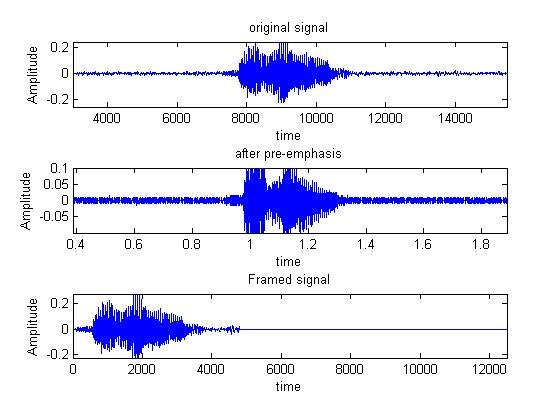
\includegraphics[width=2.9in]{figure10}
\caption{Pre-emphasis of voice signal}
\label{fig:figure10}
\end{figure}

\begin{figure}[htbp]
\centering
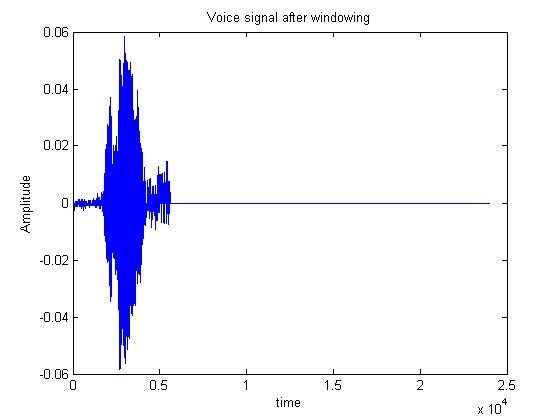
\includegraphics[width=2.9in]{figure11}
\caption{Windowing of the voice signal}
\label{fig:figure11}
\end{figure}

\begin{figure}[htbp]
\centering
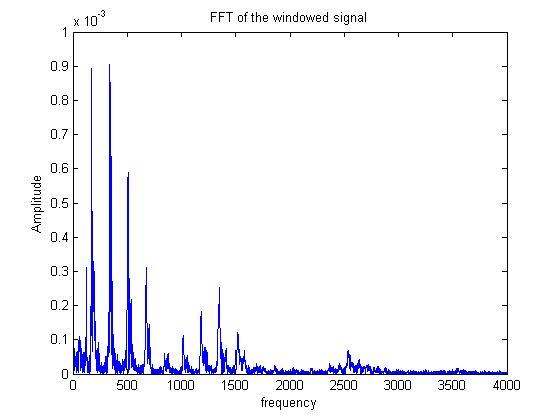
\includegraphics[width=2.9in]{figure12}
\caption{FFT of the voice signal}
\label{fig:figure12}
\end{figure}

\section{Conclusion}
We had proposed to build a system which interfaces two
important human sensing features – hearing and vision to a
robot system to provide the robot with human like capability
of understanding the voice command and recognizing the
objects shown to it. To achieve this, we extracted speech
feature using MFCC, and object feature extraction using
SURF; and implemented it in Raspberry Pi so as to make the
robot system embedded and more mobile. The extracted
features were matched with the reference database to perform
the recognition. There are still many shortages of our system,
but we are sure it could be improved and optimized in the
future.


% needed in second column of first page if using \IEEEpubid
%\IEEEpubidadjcol

% An example of a floating figure using the graphicx package.
% Note that \label must occur AFTER (or within) \caption.
% For figures, \caption should occur after the \includegraphics.
% Note that IEEEtran v1.7 and later has special internal code that
% is designed to preserve the operation of \label within \caption
% even when the captionsoff option is in effect. However, because
% of issues like this, it may be the safest practice to put all your
% \label just after \caption rather than within \caption{}.
%
% Reminder: the "draftcls" or "draftclsnofoot", not "draft", class
% option should be used if it is desired that the figures are to be
% displayed while in draft mode.
%
%\begin{figure}[!t]
%\centering
%\includegraphics[width=2.5in]{myfigure}
% where an .eps filename suffix will be assumed under latex, 
% and a .pdf suffix will be assumed for pdflatex; or what has been declared
% via \DeclareGraphicsExtensions.
%\caption{Simulation Results}
%\label{fig_sim}
%\end{figure}

% Note that IEEE typically puts floats only at the top, even when this
% results in a large percentage of a column being occupied by floats.


% An example of a double column floating figure using two subfigures.
% (The subfig.sty package must be loaded for this to work.)
% The subfigure \label commands are set within each subfloat command, the
% \label for the overall figure must come after \caption.
% \hfil must be used as a separator to get equal spacing.
% The subfigure.sty package works much the same way, except \subfigure is
% used instead of \subfloat.
%
%\begin{figure*}[!t]
%\centerline{\subfloat[Case I]\includegraphics[width=2.5in]{subfigcase1}%
%\label{fig_first_case}}
%\hfil
%\subfloat[Case II]{\includegraphics[width=2.5in]{subfigcase2}%
%\label{fig_second_case}}}
%\caption{Simulation results}
%\label{fig_sim}
%\end{figure*}
%
% Note that often IEEE papers with subfigures do not employ subfigure
% captions (using the optional argument to \subfloat), but instead will
% reference/describe all of them (a), (b), etc., within the main caption.


% An example of a floating table. Note that, for IEEE style tables, the 
% \caption command should come BEFORE the table. Table text will default to
% \footnotesize as IEEE normally uses this smaller font for tables.
% The \label must come after \caption as always.
%
%\begin{table}[!t]
%% increase table row spacing, adjust to taste
%\renewcommand{\arraystretch}{1.3}
% if using array.sty, it might be a good idea to tweak the value of
% \extrarowheight as needed to properly center the text within the cells
%\caption{An Example of a Table}
%\label{table_example}
%\centering
%% Some packages, such as MDW tools, offer better commands for making tables
%% than the plain LaTeX2e tabular which is used here.
%\begin{tabular}{|c||c|}
%\hline
%One & Two\\
%\hline
%Three & Four\\
%\hline
%\end{tabular}
%\end{table}


% Note that IEEE does not put floats in the very first column - or typically
% anywhere on the first page for that matter. Also, in-text middle ("here")
% positioning is not used. Most IEEE journals use top floats exclusively.
% Note that, LaTeX2e, unlike IEEE journals, places footnotes above bottom
% floats. This can be corrected via the \fnbelowfloat command of the
% stfloats package.





% if have a single appendix:
%\appendix[Proof of the Zonklar Equations]
% or
%\appendix  % for no appendix heading
% do not use \section anymore after \appendix, only \section*
% is possibly needed

% use appendices with more than one appendix
% then use \section to start each appendix
% you must declare a \section before using any
% \subsection or using \label (\appendices by itself
% starts a section numbered zero.)
%


% \appendices
% \section{Proof of the First Zonklar Equation}
% Some text for the appendix.

% use section* for acknowledgement


% Can use something like this to put references on a page
% by themselves when using endfloat and the captionsoff option.
\ifCLASSOPTIONcaptionsoff
  \newpage
\fi



% trigger a \newpage just before the given reference
% number - used to balance the columns on the last page
% adjust value as needed - may need to be readjusted if
% the document is modified later
%\IEEEtriggeratref{8}
% The "triggered" command can be changed if desired:
%\IEEEtriggercmd{\enlargethispage{-5in}}

% references section

% can use a bibliography generated by BibTeX as a .bbl file
% BibTeX documentation can be easily obtained at:
% http://www.ctan.org/tex-archive/biblio/bibtex/contrib/doc/
% The IEEEtran BibTeX style support page is at:
% http://www.michaelshell.org/tex/ieeetran/bibtex/
%\bibliographystyle{IEEEtran}
% argument is your BibTeX string definitions and bibliography database(s)
%\bibliography{IEEEabrv,../bib/paper}
%
% <OR> manually copy in the resultant .bbl file
% set second argument of \begin to the number of references
% (used to reserve space for the reference number labels box)
\begin{thebibliography}{1}

    \bibitem{Ahuja2013}
        K. Ahuja and P. Tuli, "Object Recognition by Template Matching Using Correlations and Phase Angle Method," 
        \emph{International Journal of Advanced Research in Computer and Communication Engineering}, 
        vol. 2, no. 3, pp. 1368-1373, 2013.

    \bibitem{Jia2008}
        T. Jia, N.L. Sun, and M.Y. Cao, 
        "Moving object detection based on blob analysis." 
        in \emph{2008 IEEE International Conference on Automation and Logistics} 
        IEEE, 2008.

    \bibitem{Schmitt2011}
        D. Schmitt, and  N. McCoy, "Object classification and localization using SURF descriptors". 
        \emph{CS, 229} (2011), 1-5.

    \bibitem{Lecun1999}
        Y. Lecun, P. Haffner, L. Bottou, and Y. Bengio, “Object Recognition with Gradient-Based Learning,” 
        \emph{Shape, Contour and Grouping in Computer Vision Lecture Notes in Computer Science}, pp. 319–345, 1999.

    \bibitem{Grauman2011}
        K. Grauman and B. Leibe, “Visual Object Recognition,” 
        \emph{Synthesis Lectures on Artificial Intelligence and Machine Learning}, vol. 5, no. 2, pp. 1–181, 2011. 

    \bibitem{Bay2006}
        H. Bay, T. Tuytelaars, and L. V. Gool, “SURF: Speeded Up Robust Features,” 
        \emph{Computer Vision – ECCV 2006 Lecture Notes in Computer Science}, pp. 404–417, 2006. 

    \bibitem{Minichino2015}
        J. Minichino and J. Howse, 
        \emph{Learning OpenCV 3 computer vision with Python: unleash the power of computer vision with Python using OpenCV}. 
        Birmingham, UK: Packt Publishing, 2015. 

    \bibitem{Alpaydin2010}
        E. Alpaydin, 
        \emph{Introduction to machine learning}. Cambridge, MA: MIT Press, 2010. 

    \bibitem{OpenCV2016}
        "OpenCV: Introduction to Support Vector Machines", 
        Docs.opencv.org, 2016. [Online]. 
        Available: http://docs.opencv.org/3.1.0/d1/d73/tutorial\_introduction\_to\_svm.html. [Accessed: 02- May- 2016].

    \bibitem{Holmes2001}
        J.  Holmes and W.  Holmes, 
        \emph{Speech synthesis and recognition}. 
        London: Taylor \& Francis, 2001.

    \bibitem{Gopi2014}
        E. S. Gopi, 
        \emph{Digital speech processing using Matlab}. New Delhi: Springer, 2014. 

    \bibitem{Raspberry2016}
        "Raspberry Pi 2 Model B", Raspberry Pi, 2016. 
        [Online]. Available: https://www.raspberrypi.org/products/raspberry-pi-2-model-b/. [Accessed: 02- May- 2016].

    \bibitem{Camera2016}
        "Camera Module - Raspberry Pi", 
        Raspberry Pi, 2016. [Online]. 
        Available: https://www.raspberrypi.org/products/camera-module/. [Accessed: 02- May- 2016].

\end{thebibliography}

% biography section
% 
% If you have an EPS/PDF photo (graphicx package needed) extra braces are
% needed around the contents of the optional argument to biography to prevent
% the LaTeX parser from getting confused when it sees the complicated
% \includegraphics command within an optional argument. (You could create
% your own custom macro containing the \includegraphics command to make things
% simpler here.)
%\begin{biography}[{\includegraphics[width=1in,height=1.25in,clip,keepaspectratio]{mshell}}]{Michael Shell}
% or if you just want to reserve a space for a photo:

% You can push biographies down or up by placing
% a \vfill before or after them. The appropriate
% use of \vfill depends on what kind of text is
% on the last page and whether or not the columns
% are being equalized.

%\vfill

% Can be used to pull up biographies so that the bottom of the last one
% is flush with the other column.
%\enlargethispage{-5in}



% that's all folks
\end{document}


